%\documentclass{report}
%\usepackage[T1]{fontenc}
%\usepackage[utf8]{inputenc}
%\usepackage[francais]{babel}
%\usepackage{amsmath}
%\usepackage{graphicx}
%\graphicspath{{Figures/}}
%\usepackage[backend=biber,style=authoryear,bibencoding=utf8]{biblatex}
%\usepackage[colorlinks,linkcolor=blue]{hyperref}
%\newcommand{\micro}{$\mathrm{\mu}$}
%\addbibresource{biblio2.bib}
%\begin{document}

\chapter{Rhéologie locale d'une cellule unique}
\begin{center}

\includegraphics[scale=0.7]{Chapitre7.png}

\end{center}
\newpage

Les pinces magnétiques ont été construites afin de pouvoir observer l'évolution des caractéristiques mécaniques d'une cellule au cours du temps, lorsque celle-ci est soumise à des forces de manière répétée. L'objectif initial était de poursuivre ainsi une investigation débutée par Delphine Icard avec les pinces optiques. En effet, dans sa thèse, elle avait observé que lorsqu'une force identique est appliquée de manière répétée sur une cellule, elle devient de plus en plus rigide, et que cet effet s'accompagne d'un recrutement d'actine autour du point d'application de la force. L'utilisation de pinces magnétiques nous permet de réaliser des expériences sous microscope confocal, ce qui n'était pas possible avec les pinces optiques. Ces expériences couplant mécanique et observations en microscopie de fluorescence seront décrites au chapitre suivant. 

Deux expériences sont décrites ici : les expériences faites avec la pince immédiatement après sa construction et donc le but est d'observer l'évolution des paramètres mécaniques de C2C12 isolées, et des expériences faites bien après en collaboration avec Pierre-Oliver Strale sur d'autres cellules exprimant des cadhérines mutantes. 

\section{\'Evolution de la rigidité de C2C12 sous l'application d'une force}

\subsection{Protocole expérimental}

\subsubsection{Séries d'expériences}

Trois séries d'expériences ont été réalisées avec les pinces magnétiques.
La première série d'expérience a été réalisée sur des C2C12 en testant deux concentrations de fibronectine pour enrober les billes magnétiques : 2 \micro g ou  4 \micro g de fibronectine pour $2.10^7$ billes, ce qui correspond à 1.57 et 3.15 mg/m$^2$ de fibronectine par unité de surface des billes, en supposant que tout s'adsorbe.  
On applique sur ces cellules 4 créneaux de force successifs de 125 secondes chacun suivi de 125 secondes de relaxation. 

La seconde série d'expériences a été réalisée sur une autre série de C2C12, issues d'une nouvelle commande à l'ATCC, avec 4 \micro g de fibronectine pour $2.10^7$ billes et 6 paliers de force de 125 secondes et de 125 secondes de relaxation. 
À la suite des expériences de la série \no 1, il nous est en effet apparu que 4 applications de force ne permettaient pas toujours de caractériser le comportement à long terme de la cellule, et nous avons donc augmenté le nombre d'applications de force. 

La troisième série d'expériences est un témoin réalisé avec les mêmes cellules que l'expérience précédente, la même quantité de fibronectine sur les billes, mais seulement 10 secondes d'application de la force, ce qui correspond au temps nécessaire pour extraire les paramètres mécaniques de la cellule. 


%Enfin les pinces magnétiques ont également servi à faire des mesures dans le cadre d'une collaboration avec Pierre-Olivier Strale et René-Marc Mège de l'Institut Jacques Monod. Il s'agissait de mesurer les caractéristiques mécaniques de cellules A431D exprimant une cadhérine mutante incapable de former des interactions cis avec d'autres cadhérines de la même membrane, et des billes enrobées de cadhérines et non de fibronectine. 


\subsubsection{Sélection préliminaire}

Une fois l'expérience mise en place comme cela a été décrit dans le chapitre précédent, la première étape consiste à trouver une bille adhérent à une cellule sur laquelle on puisse faire des mesures. 
On écarte volontairement toutes les billes qui sont trop proches d'une autre bille : en effet, lorsque deux billes sont proches, elles interagissent, et s'attirent l'une vers l'autre jusqu'à former un doublet aligné avec les lignes de champ magnétiques. Il est alors impossible de connaître précisément la force exercée sur la bille. 

Lorsque l'on repère une bille isolée adhérant à une cellule, un premier test rapide est réalisé.
On commence par appliquer une force oscillante sur la bille, et on observe si un mouvement oscillant de la bille est détectable. Si aucun mouvement n'est détectable, on augmente la force jusqu'à détecter un mouvement. Si aucun mouvement n'est détectable à la force maximale, c'est que la bille est trop fortement ancrée, ou la cellule trop rigide pour que l'on puisse mesurer ses caractéristiques à l'aide de notre dispositif. 

Il aurait été intéressant de compter le nombre de cellules écartées à cause d'une trop grande rigidité, car cela nous aurait donné un aperçu de la quantité de la population qu'il était impossible de sonder avec le dispositif tel qu'il était monté. Cela a d'ailleurs été fait dans la deuxième expérience sur les cadhérines mutées, sur un autre type cellulaire. 

\subsubsection{Sélection a posteriori}

Il arrive qu'au cours de l'expérience, lorsqu'une bille n'est que peu ancrée à la cellule, elle soit arrachée lors d'une application de la force.
Il peut également arriver que la cellule observée ait un mouvement propre tellement important qu'elle fait sortir la bille du  champ de la caméra. 

Dans ces deux cas, les expériences partielles ne sont pas dépouillées avec les autres, car il leur manque une partie de l'information, mais elles sont dénombrées.



\subsubsection{Direction du mouvement des billes}
Au temps t=0, une force constante est appliquée sur la cellule par l'intermédiaire de la bille. 

La bille est attirée par la pointe de la pince par une force $\vec{F}_{tot}=F_x \vec{u}_x+F_y \vec{u}_z$ dirigée selon l'axe bille-pointe. Comme la pointe fait un angle de 45\degres  avec l'horizontale, on a $F_y \approx F_x = F = \sqrt{2} F_{tot}$. 

Sur la vidéo, on peut observer la position dans le plan XY du centre de la bille, et constater que la bille est bien attirée par la pointe selon X et n'a qu'un mouvement faible selon Y dû aux petits défauts d'alignement de la pointe ou à la forme de la cellule (la bille contourne parfois un obstacle comme le noyau). La plupart des billes ont un déplacement total de l'ordre de 0.1 à 0.5 \micro m lors d'une application de force. 

Une fois les positions du centre de la bille extraites de la vidéo par le logiciel d'analyse d'images, on peut en tirer le déplacement de la bille par rapport à sa position au temps t=0 de l'application de la force, pour chaque créneau $\delta R(t)=\sqrt{\delta x(t)^2+\delta y(t)^2}$. 
La plupart du temps, la force dans le plan horizontal étant alignée avec l'axe X, on a $\delta R(t) \approx \delta x(t)$. Lorsque le mouvement en réponse à la force se fait également selon l'axe Y, c'est en général lié à la morphologie de la cellule, comme par exemple lorsque la bille est tirée vers le noyau et le contourne. 
 
Durant les expériences de pinces magnétiques, nous ne pouvons pas mesurer l'angle d'enfoncement des billes. Cependant, des cellules fixées ont été observées au microscope confocal, ce qui nous a permis de mesurer l'angle d'enfoncement des billes, et la hauteur $h_u$ pour 23 billes. On obtient alors : 
$$ \langle h_u \rangle = 1.6 \mu m \: \langle \theta \rangle = 110 \degres$$

On voit bien ici que l'hypothèse d'un milieu semi-infini sous la bille n'est pas du tout vérifiée. Au contraire, on a même $\frac{h_u}{2a} <1$. 

Ce qui nous donne avec les deux modèles : 
\begin{align}
 p_{Gallet}&=\frac{2}{3}\left(\frac{1}{\left( \frac{3}{2 \sin \theta}+\frac{\cos \theta}{\sin^3 \theta}\right)} \right) = 0.50 \\
p_{Kamgoue}&= 0.92\\
\end{align}

On peut également obtenir des informations sur le mouvement de la bille en Z en observant la variation de son rayon, qui augmente lorsqu'elle quitte le plan focal. 

Une calibration à l'aide d'une cale piézo-électrique a permis de déterminer qu'une variation de diamètre de la bille de 0.04\micro m correspond à une variation de hauteur de 0.2 \micro m. 
Or sur la quasi-totalité des billes observées au cours de ces expériences, la variation du diamètre des billes est inférieure à 0.02 \micro m, ce qui correspond à une borne supérieure de mouvement vertical de 0.1 \micro m de l'ordre de la borne inférieure des mouvements détectés selon l'axe X. 

La pince magnétique applique une force égale selon les deux axes X et Z, mais les déplacements mesurés dans les deux directions sont différents : les cellules semblent plus rigides dans la direction verticale par rapport à l'horizontale. 

La faible épaisseur des cellules joue probablement un rôle important dans ces différences de déformations entre l'axe vertical et le plan horizontal : il y a peu de milieu cellulaire à déformer entre la bille et la lamelle de verre. La cellule est ancrée sur cette dernière fortement par la liaison intégrine-fibronectine. L'influence de la rigidité de la lamelle de verre, quasiment infinie par rapport à celle de la cellule, peut alors être sentie lorsque l'on sonde le milieu avec la bille. 



\subsubsection{Fonction de fluage en loi de puissance}

Par défaut, la fonction de fluage sera calculée sans son préfacteur géométrique $p$, qui dépend du modèle choisi mais est strictement identique d'une expérience à l'autre ici.
$$ J(t) = 2 \pi a p \xi (t)\qquad \xi (t) = \frac{\delta x (t)}{F}$$
	
\begin{figure}
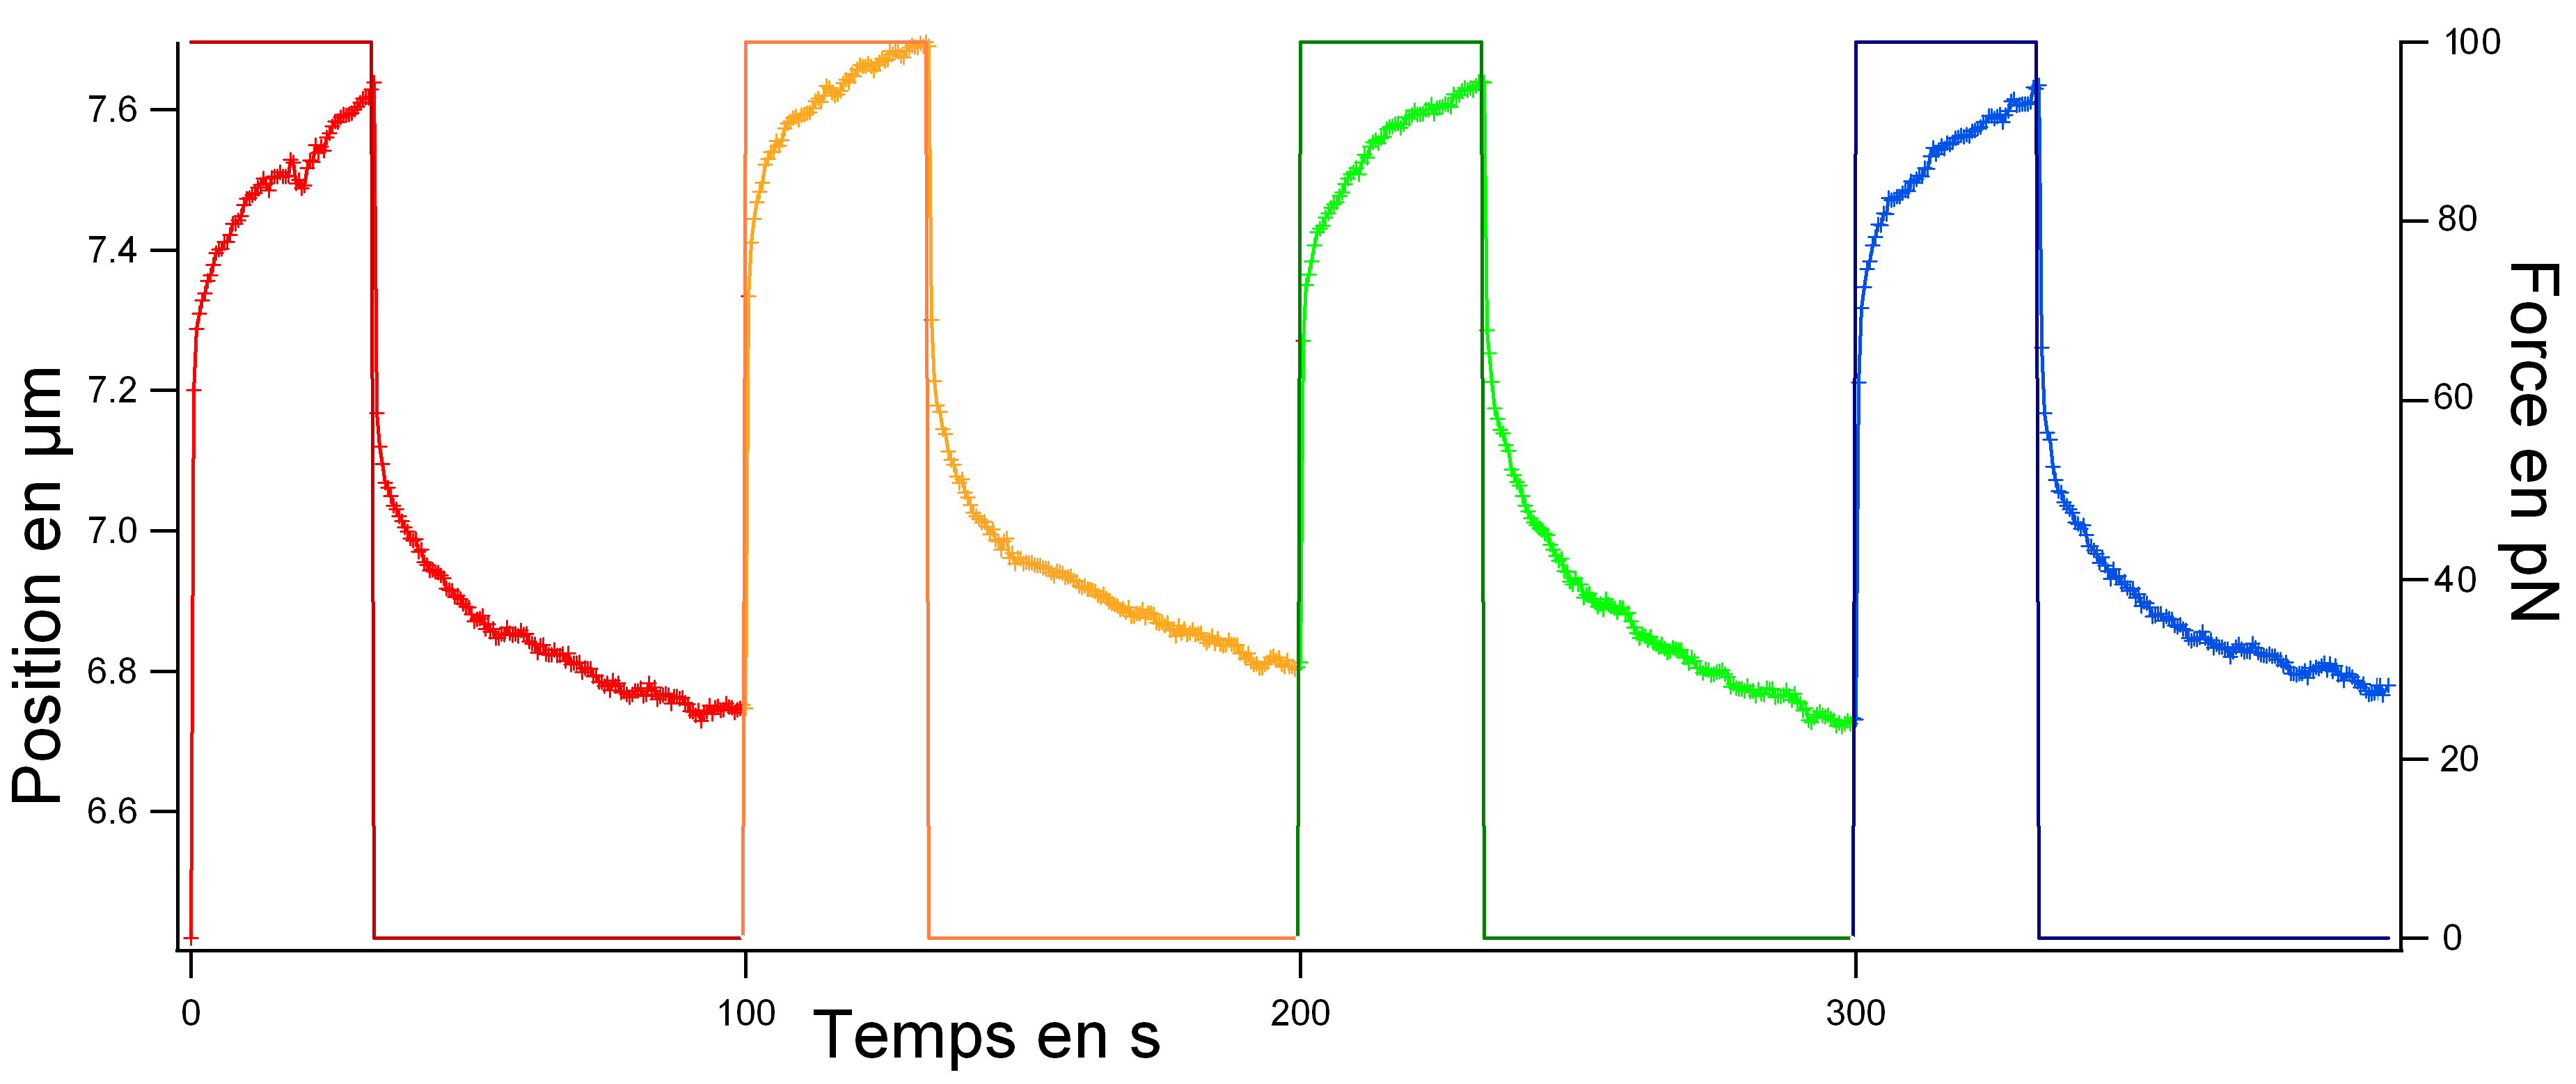
\includegraphics[scale=0.11]{c9-rigidification-couleurs.png}

\caption{Exemple de tracé de la position selon $x$ d'une bille au cours du temps lorsqu'elle est soumise à 4 créneaux de force successifs. $\delta R(t)$ =$\delta x(t)$ lorsque le déplacement ne se fait que selon l'axe $X$. On peut remarquer l'allure caractéristique en loi de puissance.\label{Exemple}} 
	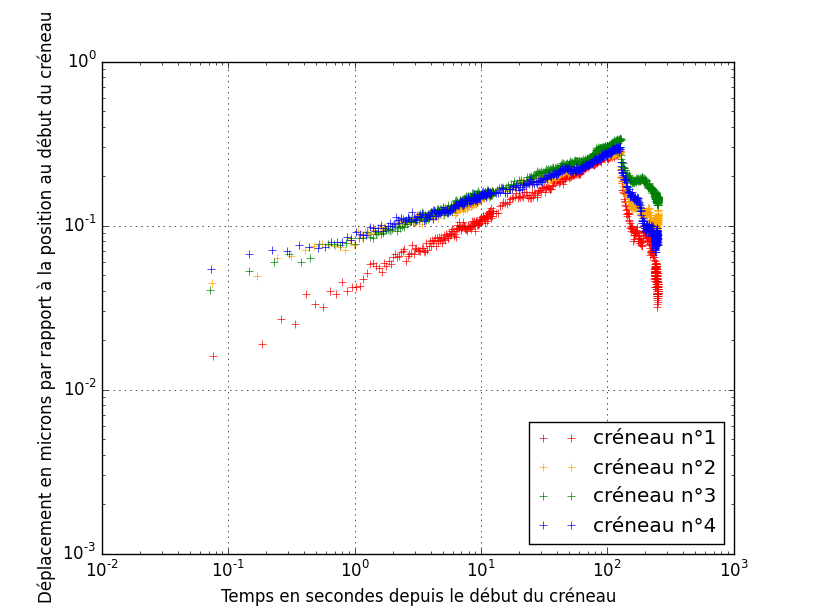
\includegraphics[scale=0.5]{Figures/Exemple_C162_loglog.png}
	\caption{Déplacement de la bille en fonction du temps écoulé depuis le début du créneau, pour les 4 créneaux successifs. On peut remarquer ici qu'après le premier créneau le déplacement est plus grand en réponse à la même force : la cellule s'est \og ramollie \fg. }
\end{figure}

	 
La fonction de fluage de la cellule peut être correctement ajustée par une loi de puissance à une échelle de temps inférieure à 15-20 secondes. Au-delà, les mouvements actifs de la cellule perturbent le mouvement de la bille.  
L'utilisation d'une loi de puissance nous permet de réaliser tous les ajustements avec seulement deux paramètres, ce que ne permettrait pas une série d'exponentielles. 

On peut alors réaliser un ajustement avec la fonction : 
$$ \xi (t) = \frac{\delta x}{F}=A \left( \frac{t}{t_0} \right)^{\alpha}$$

$A$ et $\alpha$ sont les caractéristiques mécaniques de la cellule, $t$ le temps écoulé depuis le début de l'application du pas de force, $t_0$=1s. 

%Pour un solide parfaitement élastique, la déformation en réponse à un palier de force est immédiate et constante au cours du temps, et la fonction de fluage est alors l'inverse du module d'Young.
%$$J(t)=\frac{1}{E} = 2 \pi a p \xi(t)$$
% $$J_0=\frac{1}{E} = 2 \pi a p A$$
% $$\alpha=0$$
% 
% Pour un liquide parfaitement visqueux, la fonction de fluage est alors  proportionnelle au temps écoulé depuis le début de l'application de la force : 
% $$ J(t)=\frac{t}{\eta} = 2 \pi a p \xi(t)$$
% $$J_0=\frac{t_0}{\eta} = 2 \pi a p \frac{A}{t_0}$$
% $$\alpha=1$$
 
 $A$ représente alors la déformabilité du matériau : plus il est élevé à un instant donné, plus le matériau a été déformé à force égale. 
 $\alpha$ quantifie la dépendance temporelle de cette déformation : plus il est grand, plus le matériau aura tendance à couler comme un liquide visqueux, plus il est petit et plus il se déformera comme un solide élastique. 

Un même créneau de force est appliqué 4 à 6 fois sur les billes. 
À chaque application de force, on peut extraire les paramètres $A$ et $\alpha$ et ainsi observer leur évolution au cours du temps. 


\subsection{Résultats}



\subsubsection{Caractéristiques mécaniques des C2C12}

Les C2C12 sont des cellules très diverses dans leur taille et dans leur forme, mais également en ce qui concerne les paramètres mécaniques : $A$ s'étale sur deux décades, de $7*10^{-5}$ à $9* 10^{-3}$ \micro m/pN avec une médiane à $1.22 \dot 10^{-3}$ \micro m /pN.  Avec le modèle de Gallet, cela correspond à des modules visco-élastiques caractéristiques à 1s : 
$$G_0 = \frac{(2 \pi)^{\alpha}}{\Gamma(1+\alpha)} \frac{1}{2 \pi a p A}$$ 
Ces modules vont de 12 Pa à 6 kPa avec une médiane à 87 Pa. 
Avec le modèle de Kamgoué-Ohayon, on obtient un module d'Young E allant de 4 à 546 Pa, avec une médiane à 32 Pa. Cette large distribution de valeurs, couvrant plusieurs ordre de grandeurs, n'est pas propre aux C2C12, c'est le cas de nombreux autres types cellulaires \parencite{balland_dissipative_2005}. 

L'exposant médian, $\alpha=0.18$ nous indique que la réponse mécanique des cellules est principalement élastique.


\begin{figure}
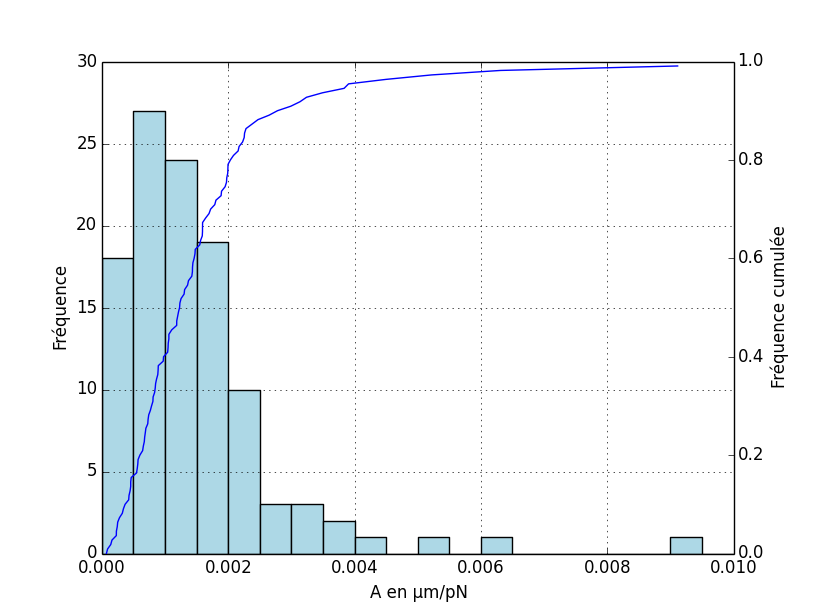
\includegraphics[scale=0.5]{Figures/A0_Toutes.png} 
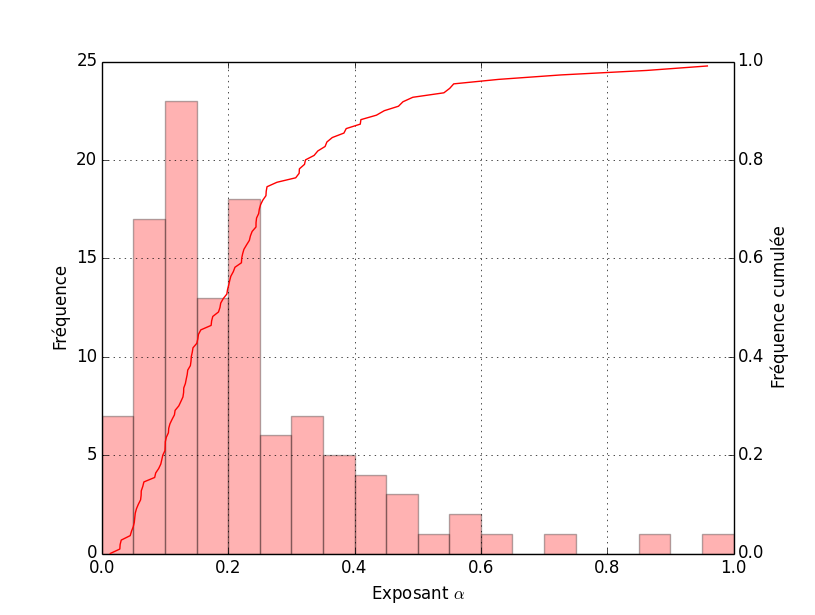
\includegraphics[scale=0.5]{Figures/E0_Toutes.png} 
\caption{Caractéristiques mécaniques des C2C12 avec 4 \micro g de fibronectine.}
\end{figure}
 
  
Il est important de rappeler que la population est tronquée de ses cellules les plus rigides.. 
Les valeurs obtenues peuvent paraître faibles en comparaison de celles obtenues précédemment sur la même lignée par Delphine Icard avec les pinces optiques. Cependant les pinces optiques opéraient sur des billes bien moins enfoncées à l'intérieur de la cellule, avec une épaisseur sous la bille plus élevée. Les éléments du cytosquelette qui entrent en jeu dans la visco-élasticité ne sont peut-être pas les mêmes. De manière générale, on voit que les valeurs de modules visco-élastiques sont très variables d'un modèle à l'autre. 

\subsubsection{Influence de l'enrobage des billes en fibronectine}

Pendant la première série d'expériences, des billes enrobées de deux concentrations différentes de fibronectine ont été utilisées. 

On peut voir en observant les deux populations que $A$ est plus élevé lorsque l'enrobage est moins dense, alors que l'exposant ne varie pas, mais cette élévation n'est pas significative avec la quantité de cellules que nous avons observées.
Lorsque la quantité de fibronectine sur les billes est plus faible, les cellules apparaissent donc comme plus déformables, moins rigides, ce qui s'explique facilement par un ancrage moindre de la bille au cytosquelette de la cellule.  Cependant, il est également possible que les billes recouvertes de moins de fibronectine soient également moins enfoncées dans les cellules, ce qui conduirait à sous-évaluer la rigidité des cellules. Seule l'observation en microscopie confocale de l'angle d'enfoncement des billes avec la quantité de fibronectine la plus faible nous permettra de trancher entre ces deux hypothèses. 

En revanche, l'équilibre entre l'élasticité et la dissipation dans la cellule n'est pas altéré : on sonde toujours le même cytosquelette, mais avec un attachement ou un enfoncement moins élevé. 

\begin{figure}
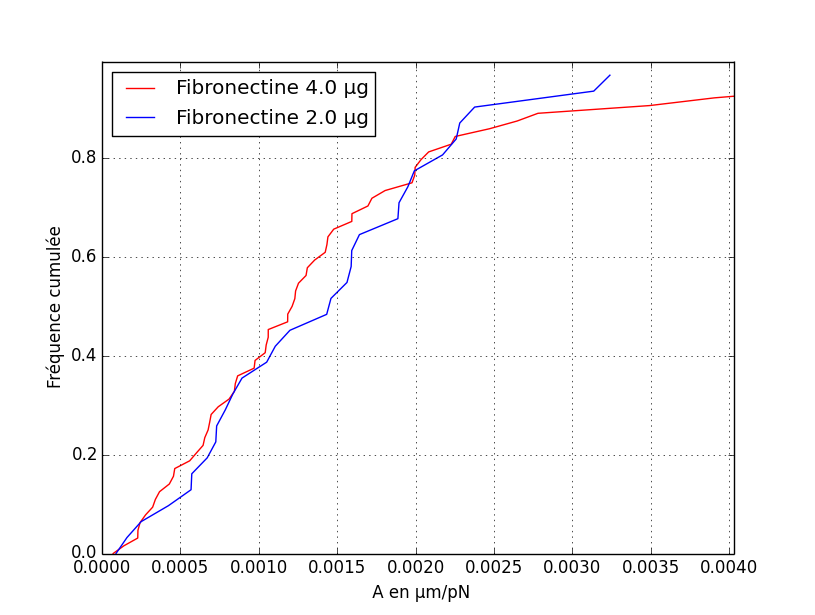
\includegraphics[scale=0.5]{Figures/A_coating_seul.png} 
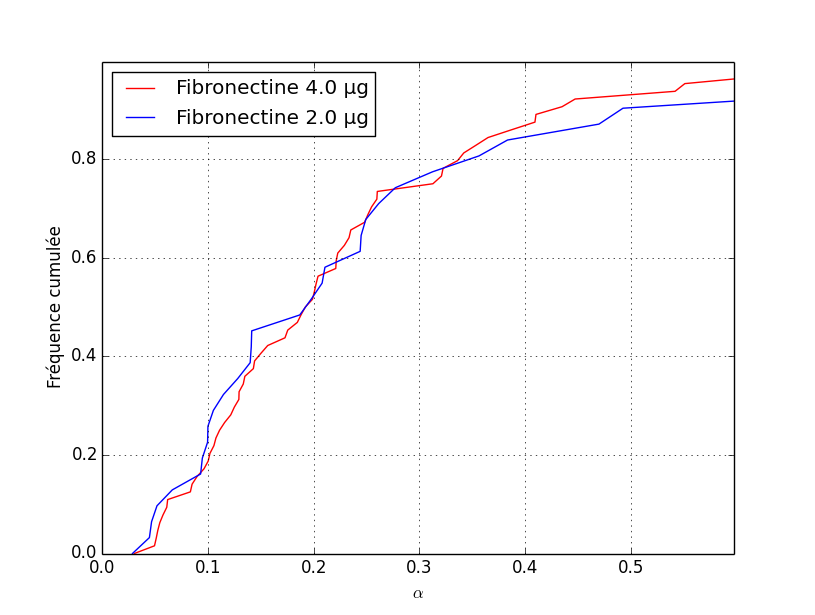
\includegraphics[scale=0.5]{Figures/E_coating_seul.png} 
\caption{Caractéristiques des C2C12 sondées par des billes ayant différentes densités de fibronectine à leur surface. p=0.13}
\end{figure}

\subsubsection{\'Evolution des paramètres mécaniques}

Pour chaque cellule, la force est appliquée à 4 reprises pour la série \no 1 et à 6 reprises pour les séries \no 2 et \no 3. On obtient alors un couple de paramètres ($A,\alpha$) par créneau, dont on observe l'évolution. 

Dans les résultats finaux, ne sont conservées que les cellules pour lesquelles la mesure des paramètres ($A, \alpha$) est possible lors de l'application du premier créneau. 
En revanche, il arrive pour un nombre non négligeable de cellules que le déplacement de la bille pendant les créneaux suivants passe en dessous de notre résolution, ce qui signifie que la cellule devient trop rigide. Dans ce cas de figure, $A$ a été fixé à 0. 

\begin{figure}
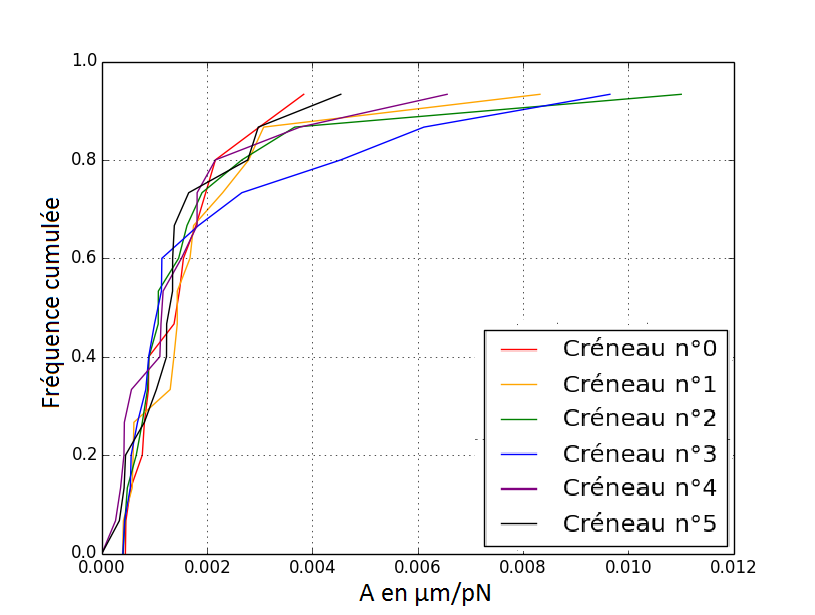
\includegraphics[scale=0.3]{Figures/A_creneaux_temoin.png}
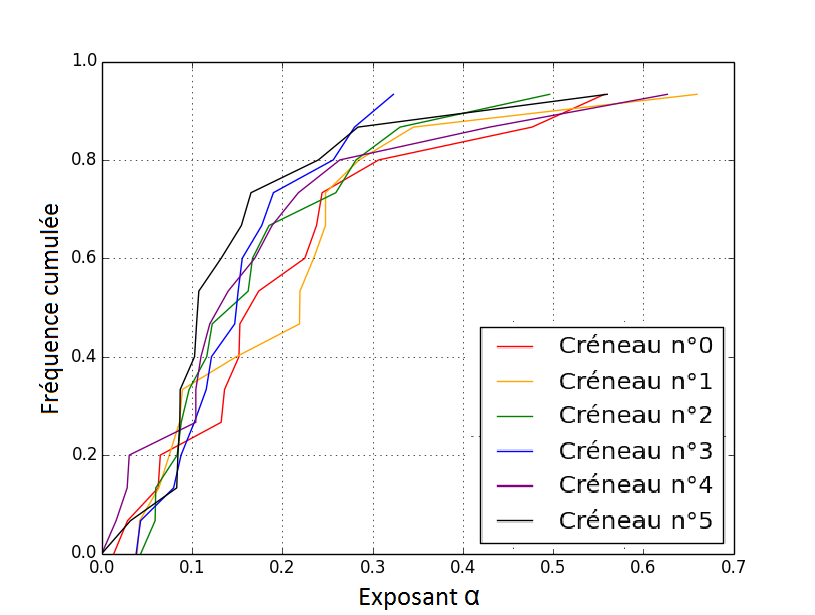
\includegraphics[scale=0.3]{Figures/E_creneaux_temoin.png} 
\\
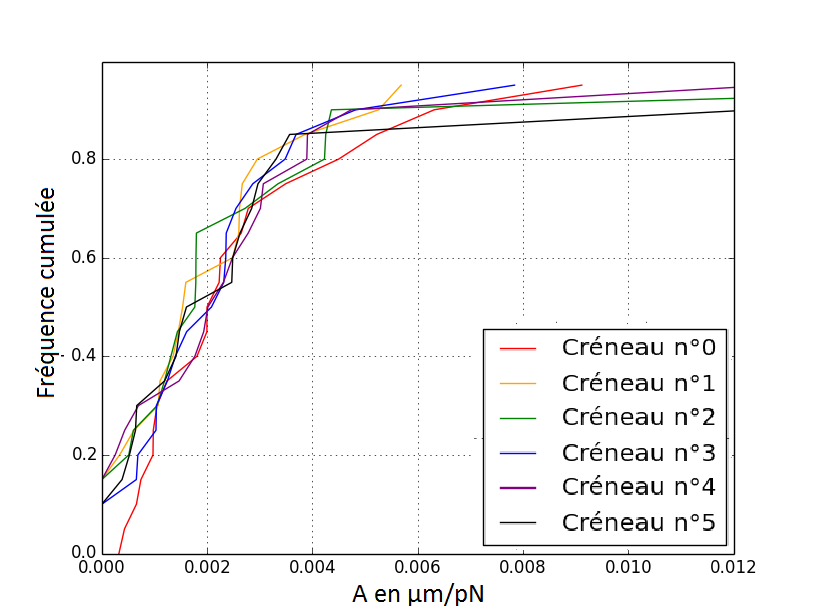
\includegraphics[scale=0.3]{Figures/A_creneaux_S2.png} 
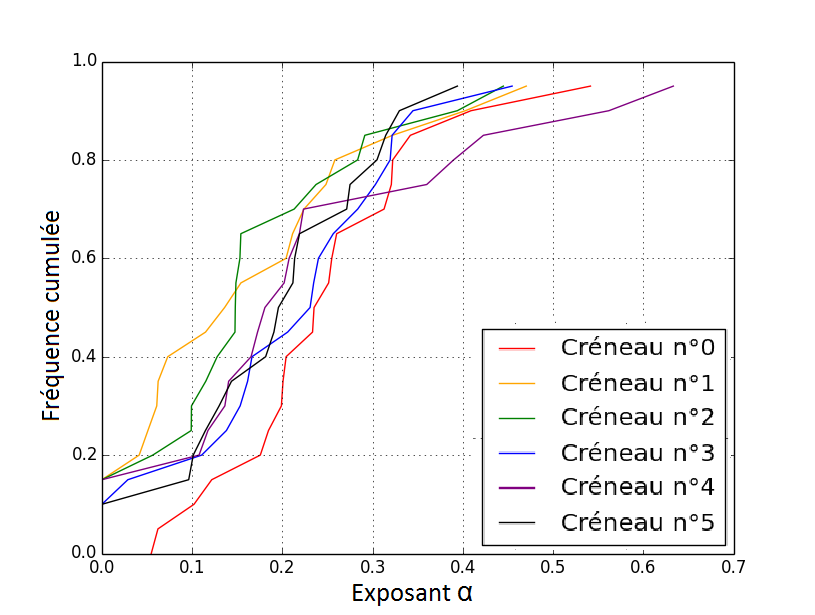
\includegraphics[scale=0.3]{Figures/E_creneaux_S2.png} 
\caption{\label{Evolution_6c}} 
\end{figure}

\begin{figure}
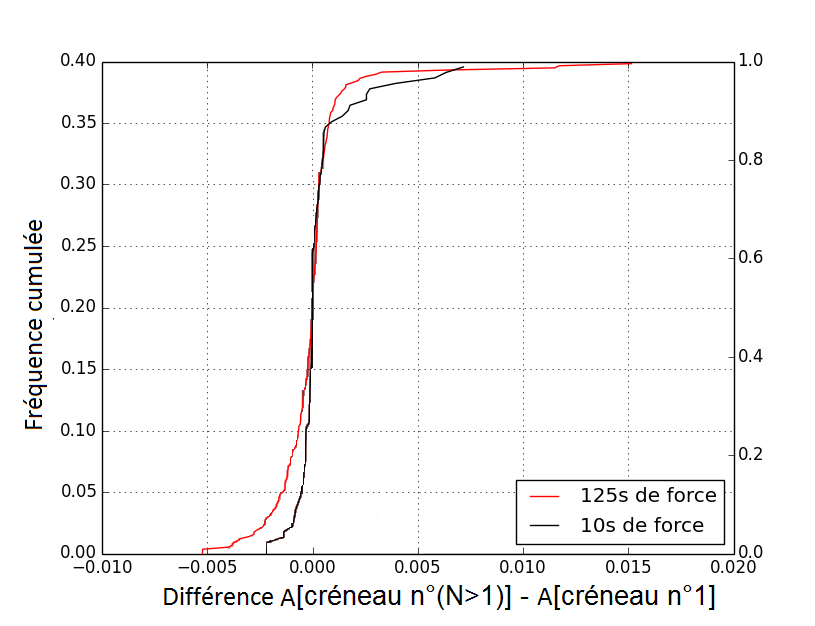
\includegraphics[scale=0.3]{Figures/A_diff_seul.png} 
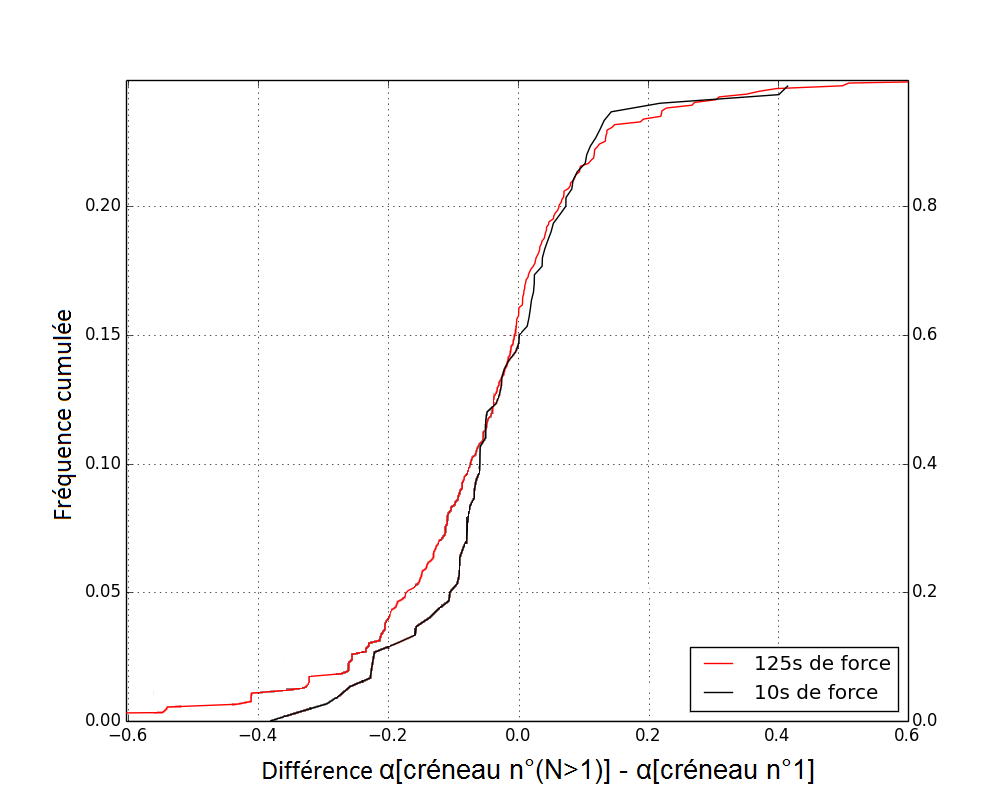
\includegraphics[scale=0.3]{Figures/E_diff_seul.png}
\caption{Amplitude des évolutions entre la première mesure et les 6 suivantes, pour la série \no 3 témoin (en noir) et pour la même concentration de fibronectine et 125s de force en rouge.}
\label{Diff}

 
\end{figure}
On peut voir sur la figure \ref{Evolution_6c} qu'il n'y a pas de changements de $A$ communs à toute la population de cellules : ce ne sont pas toutes les cellules qui se rigidifient ou se ramollissent ensemble. 
En revanche, on peut observer un décalage des exposants vers les valeurs les plus faibles aux 2\ieme  et 3\ieme créneaux, qui se résorbe ensuite, mais il n'est pas significatif. 
Le comportement mécanique de ces cellules soumises à une force pendant de longues durées évolue donc d'abord dans le sens d'une \og élastification \fg , d'une diminution de la part dissipative de la réponse mécanique. 

Lorsque l'on applique une force pendant 125 secondes, l'amplitude des variations par rapport à la mesure d'origine de $A$ et $\alpha$ se détache du bruit obtenu pour seulement 10 secondes de forces, comme on peut le voir sur l'histogramme \ref{Diff}. L'application d'une force pendant une durée plus longue permet donc de modifier significativement les paramètres $A$ et $\alpha$. 

\subsubsection{Classification des cellules selon l'évolution de leurs paramètres mécaniques}

Il n'y pas de tendance d'évolution de la population de cellules sondée au cours du temps, cependant on peut observer au niveau individuel l'évolution de $A$ pour en déduire une tendance au ramollissement ou à la rigidification. 

On classe ainsi les cellules en trois groupes : celles qui se rigidifient, avec $A$ décroissant significativement sur les 4 à 6 applications de force, celles qui se ramollissent $A$ croissant significativement sur les 4 à 6 applications de force, et celles qui n'ont pas une évolution significative ou cohérente dans le temps de $A$. 
On peut créer un classement semblable avec l'évolution de l'exposant $\alpha$. 
\begin{figure}
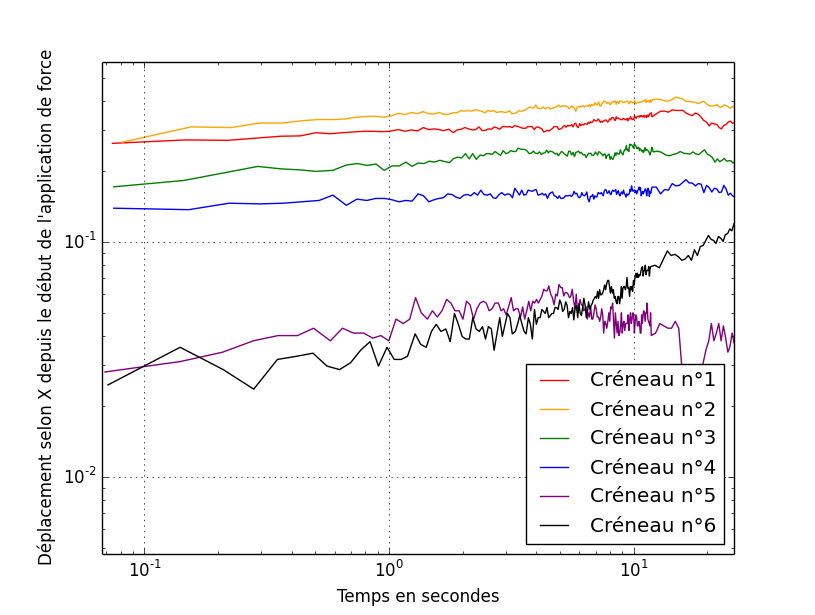
\includegraphics[scale=0.33]{Figures/Rigidification_exemple_s2c2.png} 
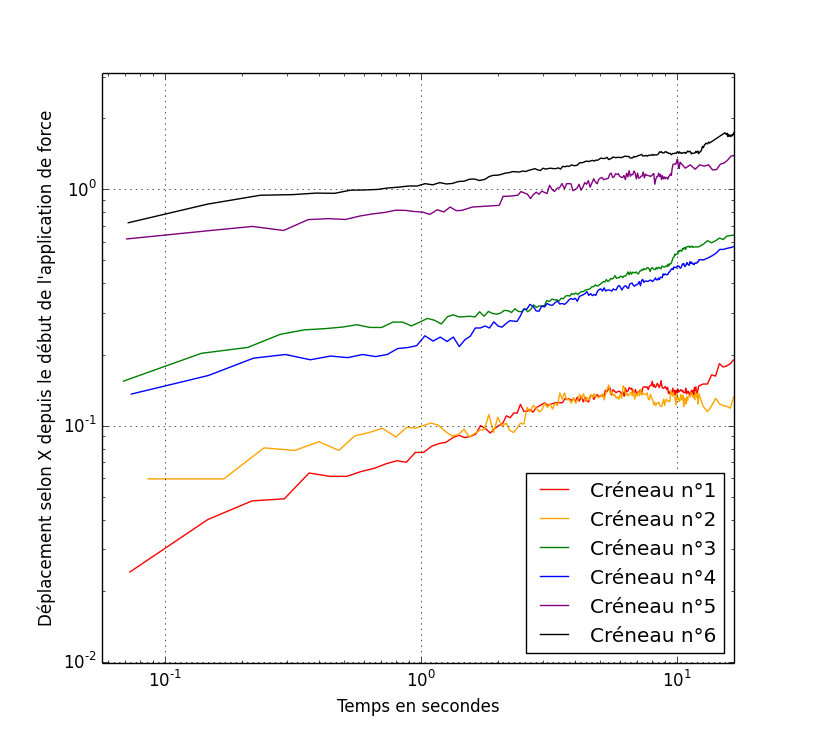
\includegraphics[scale=0.3]{Figures/Ramollissement_exemple_s2c19.png} 
\caption{Exemples de déplacements au cours du temps et au cours des applications de forces d'une cellule considérée comme en rigification (à gauche) et d'une cellule en ramollissement (à droite). }
\end{figure}

\begin{figure}
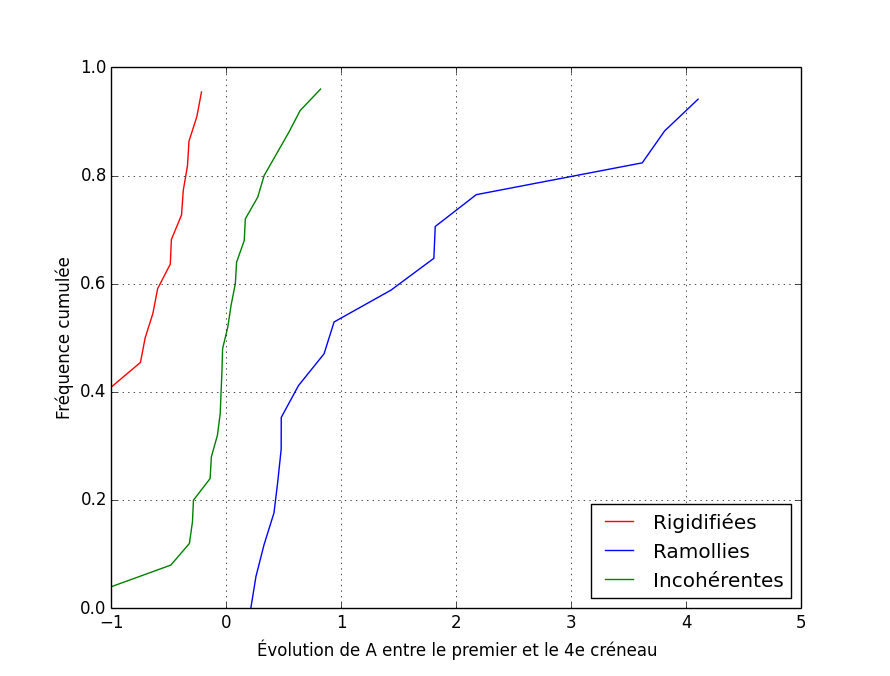
\includegraphics[scale=0.5]{Figures/Evolution_J4-J0_sur_J0.png} 
\caption{Histogramme cumulé de $\frac{A_4-A_1}{A_1}$ pour les trois groupes de cellules classées. On voit que près de la moitié des cellules se rigidifiant sont passées sous le seuil de détection de la pince, tandis que les ramollissements sont souvent supérieurs à 100\%.  }
\end{figure}

\begin{figure}
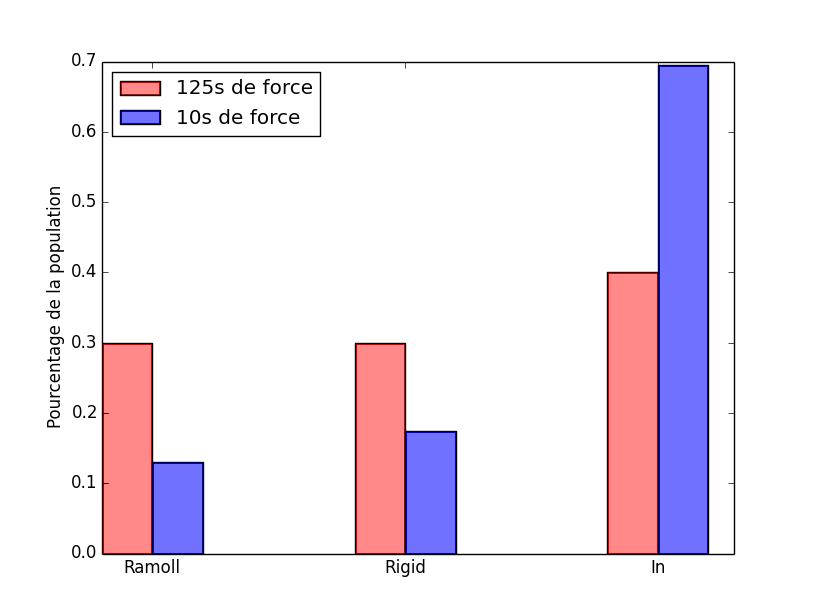
\includegraphics[scale=0.5]{Figures/FRI_temoin_vs_C4.png} 
\caption{Répartition des cellules dans les trois catégories d'évolution de $A$ au cours des applications de force \label{FRI_temoin}}
\end{figure}

On peut remarquer sur la figure \ref{FRI_temoin} que lorsque la force n'est appliquée que durant 10 secondes, les cellules ont majoritairement un comportement incohérent .
Cette évolution aléatoire, et de plus de faible amplitude comme on le voit sur la figure \ref{Diff}, est très probablement le bruit sur la mesure de $A$. 

Lorsque la force est appliquée pendant 125 secondes, on peut au contraire observer qu'il y a beaucoup plus de cellules qui se ramollissent ou se rigidifient de manière persistante au cours du temps, avec une amplitude de variation plus grande que pour le témoin. 

\subsubsection{Influence de la position de la bille sur la cellule sur l'évolution des propriétés mécaniques}

On peut donc constater que parmi les cellules soumises à 125 secondes de force de manière répétée, 60\% ont une évolution cohérente de $A$ vers la rigidification ou le ramollissement et 40\% une évolution incohérente. 

Cette évolution dépend de la valeur initiale de $A$ : ce sont les cellules les plus molles initialement qui se rigidifient, et inversement. Mais cette dépendance peut être artificielle : les cellules déjà rigides qui se rigidifient n'ont pas de mouvement visible sur lequel faire des mesures, et les cellules molles qui se ramollissent finissent par voir leur bille arrachée, ou sortir du champ d'observation. 

Nous avons alors cherché si ces différences de comportement ne provenaient pas de la position de la bille sur la cellule, et de la direction selon laquelle on appliquait la contrainte. 

%Il n'y pas de différence significative entre la distance dans le plan focal entre le bord de la bille et le bord du noyau (qui peut être négative si la bille est au-dessus du noyau) des trois différentes populations de cellules. 


\begin{figure}
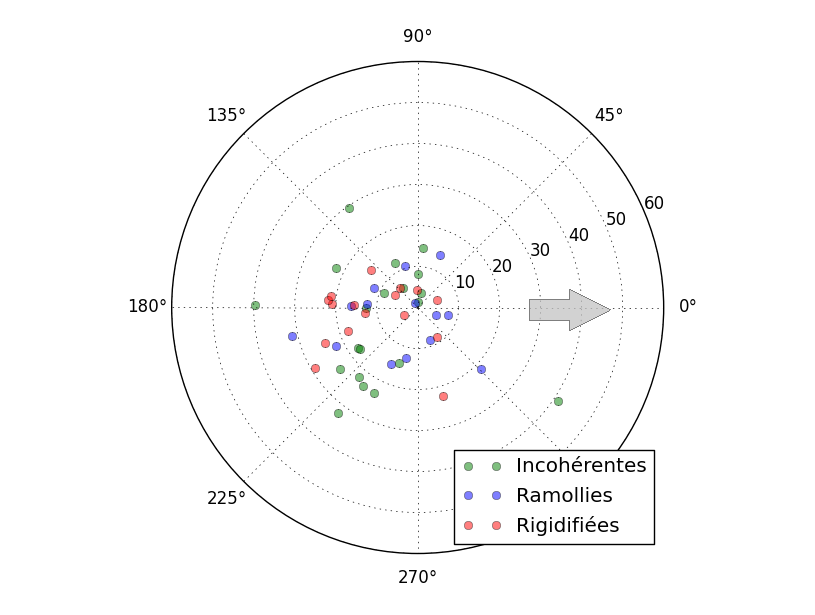
\includegraphics[scale=0.5]{Figures/Positions_FRI.png} 
\caption{Longueur et orientation du vecteur entre le bord du noyau et la bille. La flèche représente la direction de la force exercée sur les billes.\label{polar}}
\end{figure}
\begin{figure}
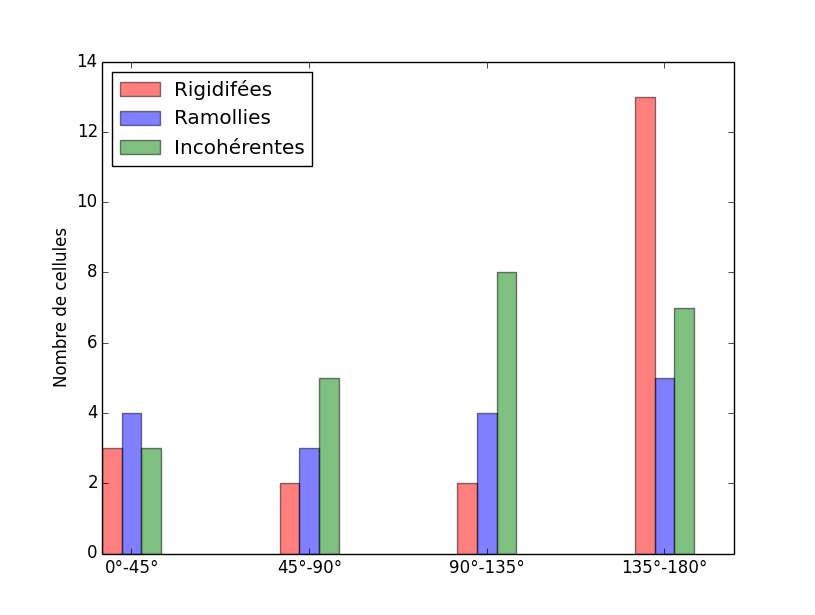
\includegraphics[scale=0.5]{Figures/Hist_Angles.png} 
\caption{Réparition des comportements cellulaires en fonction de l'angle formé entre l'axe bille-noyau et la direction de la force appliquée, pour 125 secondes de force et 4 \micro g de fibronectine. p=0.044 \label{Angle_C4}}
\end{figure}

On peut observer une corrélation entre la position de la bille par rapport au noyau et l'appartenance à l'une des trois populations, comme mis en évidence sur les figures \ref{polar} et \ref{Angle_C4}. 
Plus précisément, lorsque les billes sont \og à l'arrière du noyau \fg par rapport à la force appliquée, c'est-à-dire lorsqu'on a tendance à pousser la bille vers le noyau, alors la tendance est nettement à la rigidification. Au contraire, lorsque l'axe bille-noyau est perpendiculaire à la direction de la force, il n'y a pas de tendance cohérente. 

Au vu de cette information, on pourrait se dire que les cellules rigidifiées, qui sont tirées vers le noyau, expérimentent en fait un gradient de viscosité en se rapprochant du noyau : elles se rapprochent d'une zone péri-nucléaire où la viscosité serait plus élevée. 

Cependant, on peut voir sur la figure \ref{DBN} que ce n'est pas le cas, au contraire : la majorité des cellules qui se ramollissent se rapprochent du noyau, alors que les cellules rigidifiées se rapprochent ou s'éloignent dans des proportions égales. La statistique n'est cependant pas assez riche pour que l'on puisse affirmer que cet effet est systématique.

\begin{figure}
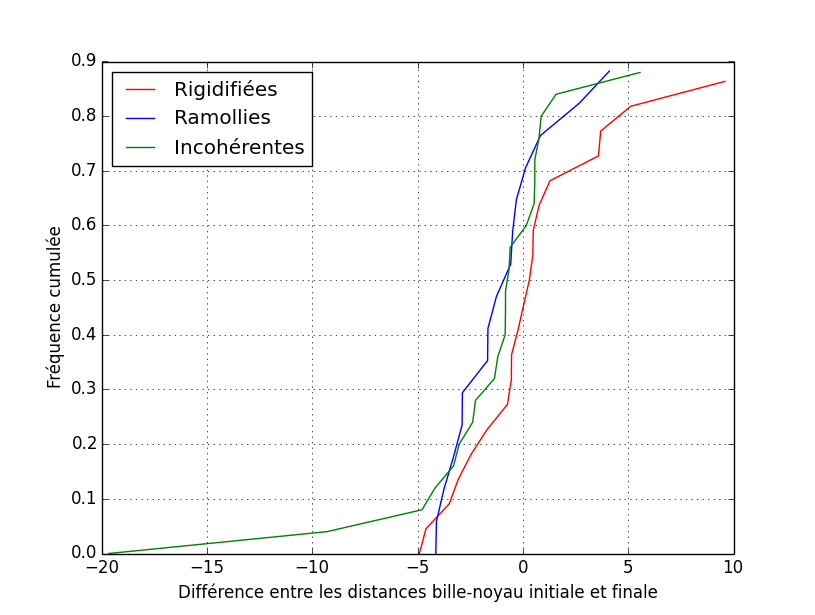
\includegraphics[scale=0.5]{Figures/Evolution_DBN.png}
\caption{Différence entre la distance bille-noyau finale et la distance bille-noyau initiale, pour les cellules classées précédemment. \label{DBN}}
\end{figure}

 
 \section{Rôle des interactions \textit{cis} des cadhérines dans la formation de contacts intercelluaires}
 
 Pierre-Olivier Strale, dans l'équipe de René-Marc Mège Adhésion Cellulaire et Mécanique de l'Institut Jacques Monod, s'est intéressé à l'oligomérisation des E-cadhérines lors de la formation des jonctions \textit{adherens}. En plus des interactions \textit{trans} qui lient les cadhérines de deux cellules différentes, les cadhérines peuvent également former des interactions \textit{cis} entre protéines appartenant à une même cellule. Elles peuvent ainsi former des agrégats à la surface de la cellule. Pour étudier le rôle de ces agrégats, ils ont conçu une cadhérine mutante, capable de former des interactions \textit{trans} mais pas des interactions \textit{cis}. La cadhérine sauvage et la cadhérine mutante étaient ensuite transfectées dans des cellules épithéliales humaines A431, qui avaient été modifiées pour ne pas exprimer l'E-cadhérine.  
 
 Ensemble, nous avons testé mécaniquement à l'aide des pinces magnétiques les propriétés des cadhérines mutantes par rapport aux cadhérines sauvages. Pour cela, on a utilisé des billes similaires à celles utilisées pendant les expériences précédemment décrites (des Dynabeads d'Invitrogen), mais de diamètre 2,8 \micro m. Ces billes pouvaient être fonctionnalisées avec une E-cadhérine sauvage. 
 
 Nous avons appliqué sur les cellules les même paliers de force périodiques que décrit dans la section précédente, avec 6 paliers par cellule. Comme indiqué dans le chapitre précédent, avant d'appliquer ces paliers de force, nous avons procédé à un test pour choisir le bon niveau de force à appliquer. 
 
 La première différence entre les cellules exprimant l'E-cadhérine mutante et celles exprimant l'E-cadhérine sauvage apparaît dès cette étape : les premières  sont significativement plus faciles à déplacer que les secondes. Nous avons classé les cellules en trois catégories : celles pour lesquelles la bille reste immobile, même en appliquant le plus haut niveau de force possible (qui est d'une vingtaine de pN ici), celles pour laquelle la bille est mise en mouvement, et celles pour lesquelles la bille a été arrachée pendant le test. Les billes sur les cellules exprimant la cadhérine mutante ont été moins souvent immobiles et plus souvent arrachées que les billes sur les cellules exprimant la cadhérine sauvage. On voir donc dès le départ que l'ancrage de la bille par les cadhérines mutantes est compromis. 
 
 Le seconde différence et visible lors de l'observation des déplacements de la bille. Lorsque la bille est ancrée par des cadhérines mutantes, son déplacement sur les 6 créneaux de force est deux fois plus important que lorsqu'elle est ancrée par les cadhérines sauvages. En revanche, dans un cas comme dans l'autre, aucune augmentation ni diminution cohérente n'a été observée. Les cellules exprimant la cadhérine mutante apparaissent donc comme moins rigides lorsqu'elle sont sondées par les jonctions \textit{adherens}. 
 
 Enfin, une troisième différence est visible lors de la phase de relaxation : les billes ancrées par des cadhérines mutantes sont beaucoup plus mobiles que les autres. Cela révèle un lien plus faible entre les cadhérines mutantes et le cytosquelette sous-jacent. 

 \begin{figure}[h!]
\caption{\small Résultats des expériences sur les E-cadhérines mutantes incapables d'interactions \textit{cis}, d'après \cite{Strale}. A : Montage expérimental, B : Proportion des billes immobiles, mobiles ou arrachées sous force pour des cellules exprimant la cadhérine mutante (cis Ecad, 54 cellules) ou sauvage (wt Ecad, 39 cellules). C : Déplacements des billes sous force en fonction du temps. D : Moyennes des déplacements pour toutes les applications de force, pour 12 billes dans chaque condition. E : Trajectoires (en \micro m) d'une bille pendant les six périodes de relaxation dans les deux conditions. F : Déplacement quadratique moyen pendant la relaxation pour 12 billes et 6 créneaux dans chaque condition}
\end{figure} 
     
 \begin{figure}
 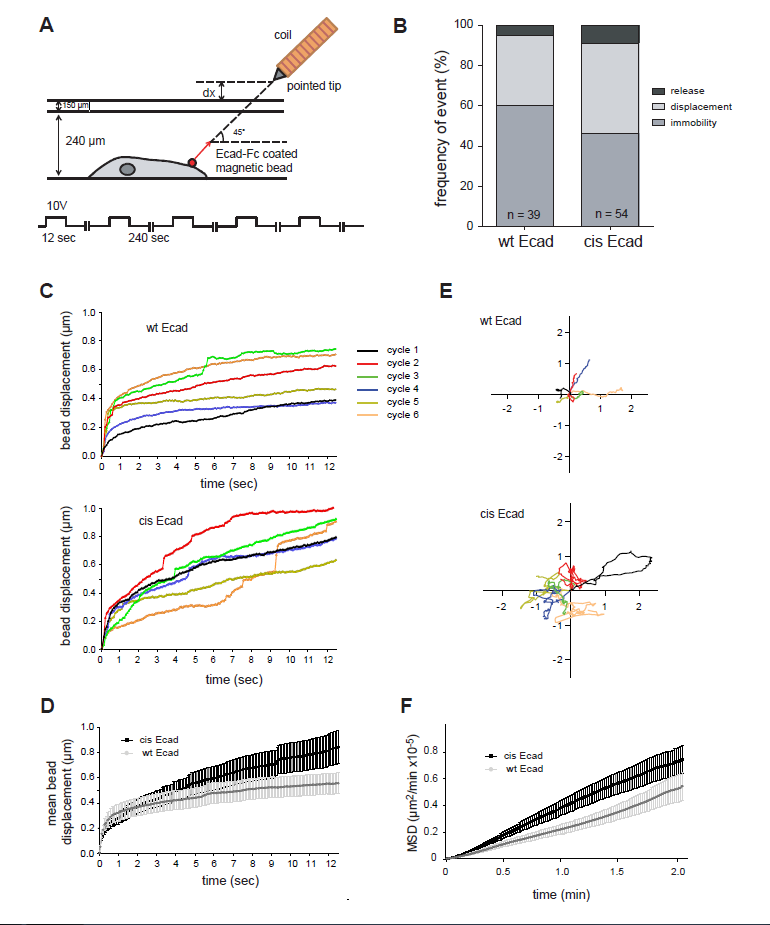
\includegraphics[scale=0.7]{Figures/Strale.png} 

 \end{figure}


 
 
 
 
%\end{document}